\begin{abstract}
Expertly operated frontier AI delivered four complete analytical recovery packages on prospective public-code cases, and a transparent commercial model supports a positive conditional business result. Each recovered notebook passed a separately authored checker on two clean-process reruns: all 133 confirmation code cells were accounted for and 38 distinct numerical and semantic checks passed. At \$900 per finally accepted package, eight attempted orders per month and 85\% final acceptance, the twelve-month model yields \$73,440 accepted revenue, \$40,309 operating profit and \$36,309 after \$4,000 additional development. The equivalent central human-service reference is an explicit eight-hour estimate at a documented \$149 hourly rate, or \$1,192. The complete-project break-even price is \$441.26 at the central volume and quality. These results answer the commercial question conditionally, without requiring scientific novelty or retained Alpha. The engineering sample consists of licensed historical teaching notebooks; a free updated edition exists, so these examples do not demonstrate demand for paid recovery. The proposed market is customer-specific analysis without an equivalent replacement. Customer demand, acceptance probabilities, acquisition expense and service-level performance remain unmeasured; actual collections are zero and complete actual study cost is unknown. A joint downside loses \$28,943, and 44.9\% final acceptance gives a \$78.66 loss under otherwise central conditions. We preserve failures and corrections, execute existing provenance and work-plan components, and provide a reproducible study, full assumptions, cash ledgers and publication sources. The supported conclusion is useful delivery with a feasible conditional commercial foundation, not a demonstrated live enterprise or an exclusive technical breakthrough.
\end{abstract}

\section*{Executive finding}
\addcontentsline{toc}{section}{Executive finding}
\textbf{The commercial arrangement works in the central modeled case.} The technical work needed to make the offering concrete was also performed: six code-only recovery packages, including two development cases and four prospective confirmation cases, are delivered with their original inputs, changes, rerun commands and evidence. Optional advantages---a new scientific principle, superiority over all conventional tools, retained skills or self-acceleration---are not used as gates that erase this result.

The strongest defensible result has two parts. First, the four confirmation analyses execute completely and pass independent checks. Second, the specified service produces positive surplus under disclosed assumptions about customers, final acceptance and full costs. Neither part establishes the other automatically. A useful construction does not prove willingness to pay; a positive model does not convert technical test cases into customer orders.

\begin{table}[htbp]\centering\small
\begin{tabularx}{\linewidth}{@{}p{.27\linewidth}Yp{.22\linewidth}@{}}\toprule
Evidence class & Result & Interpretation\\\midrule
Executed & Four fresh notebooks; 133 code cells; two clean independent reruns & Complete code paths, not four paid jobs\\
Measured & 38 distinct numerical/semantic checks; 24 identity/scope checks; adverse rejection controls & Internal engineering acceptance\\
Modeled & \$36,309 complete-project surplus at the central offer, demand and quality & Conditional commercial foundation\\
Observed financial & Zero customers, zero collections; actual complete cost unknown & No earned-revenue or actual-profit claim\\
Unestablished & Operational Alpha, retained Alpha, technical novelty, paid demand and production qualification & Separate potential advantages\\\bottomrule
\end{tabularx}
\caption{A compact evidence boundary. Repeated checks are not additional jobs or independent customers.}
\end{table}

The decisive commercial assumptions are \$900 per finally accepted capsule, 96 attempts over twelve modeled selling months, 85\% acceptance after corrections and refunds, \$125 acquisition expense per attempt, \$900 monthly attributable operations and \$4,000 additional setup. The human reference is a transparent resource estimate, not a quotation or measured human control. All amounts are USD, before income tax. No token issuance, treasury appreciation or hypothetical financing proceeds enter revenue.

\tableofcontents
\clearpage

\section{The opportunity: make inherited analytical work usable}
\subsection{A consequential restriction}
A small research or R\&D team can possess the code behind an analysis while being unable to use it. The notebook may depend on removed library interfaces, an undocumented data download, an unavailable original operator or historical defaults. Reading the result is then much easier than rerunning, checking or extending it. The potential productive gain is access to an inherited analytical capability: another question can be investigated without first building a software-maintenance function.

This is a real engineering burden, rather than an inferred market size. \citet{samuel2024} attempted 15,817 dependency-declared Python notebooks associated with biomedical publications. Dependencies installed for 10,388; 1,203 ran without errors, and 879 reproduced recorded results. These denominators describe that study's pipeline and corpus. They neither estimate the present service's success probability nor establish a buyer's budget. They support investigating the restriction: published computational work is often difficult to reuse.

\subsection{What changed, and what did not}
Frontier models can now participate directly in source interpretation, tool execution, error diagnosis, semantic repair, verification and packaging. The documented GPT-6 Astra model supports complex reasoning, coding and computer use; the present study uses the frontier assistant and authorized local tools available in this session, with its billing/configuration boundary disclosed in Section~\ref{sec:model}. The enabling hypothesis is that expert operation can reduce the repeated engineering effort of small, heterogeneous tasks enough to offer a bounded outcome at an attractive price. It is an economic possibility, not a claim that notebook modernization was just invented.

Strong alternatives already exist. Human research-software engineers perform this work. Binder supports prepared executable repositories; ReproZip captures dependencies of executions; Code Ocean checks mechanical reproducibility of submitted capsules. Code Ocean explicitly distinguishes those checks from deciding whether outputs match a published article's claims. MLEModernizer is an agentic modernization system with execution feedback. These alternatives limit differentiation and should shape pricing and scope, not function as an automatic veto of the commercial hypothesis \citep{vanderbilt,binder,reprozip,codeocean,modernizer2026}.

The most relevant current comparison is sobering. The September 2026 Waterloo author seminar reports that MLEModernizer recovered 3,292 of 8,210 failed notebooks with GPT-5.2 (40.1\%) and 3,683 with GPT-OSS-120b (44.9\%). An earlier 74.2\% headline is not used: the revised account is materially less favorable. The systems, tasks and acceptance criteria are not matched to this study. We therefore use the newer figures as adverse reference points, not as estimates of our screened service or evidence that our four cases outperform prior work \citep{modernizer2026}.

\subsection{Selection, rather than a prescribed application}
The bounded search compared three candidate needs: recovery of custom analytical notebooks; accessible STEM-diagram bundles; and reuse of legacy analytical-instrument data. Each has a plausible beneficiary and a first digital artifact. The diagram offering required actual reader-comprehension feedback to substantiate accessibility. The instrument-data offering required representative metadata and independent calibration to substantiate meaning. Those decisive resources were unavailable. Notebook recovery allowed useful construction and direct numerical checking immediately, with no laboratory, private dataset or external purchase as a critical dependency.

Selection was based on deliverability, verifiable usefulness, scope-matched labor economics and a cheap falsifier. It was not based on the exotic character of the application. The selected offer can fail in at least three inexpensive ways: the data or rights are unavailable; the intended outputs cannot be preserved or independently checked; or the buyer already has a cheaper adequate alternative. Appendix~\ref{app:shortlist} records all candidate fields and deferred evidence needs. The search is an explicit, small opportunity investigation. It does not establish universal foresight superiority.

\subsection{Relationship to the existing AGI ALPHA studies}
\citet{transformational} distinguishes intended purpose from restrictive formulations and requires an executable bridge from a change to a useful outcome. \citet{economy} adds voluntary participation, complete economics and liquidity. Their illustrative causal and shared-construction results remain in their original scope. In particular, an unrestricted conventional planner matched the former's illustrative intervention, and the latter's favorable commercial quantities were supplied-model results. None of those financial outcomes is imported into this offering.

The repository and issue~4850 were inspected at main commit \path{3947e4ec8fd74ad40e13e8ff825a149fa98a10e9}. Current archive-claim and numerical boundary-repair work remain separate. This study adds an independent path and preserves the active publisher and release lease. It neither reruns nor revises the earlier kinetics, archive or numerical conclusions. Prior useful engineering can coexist with failed novelty or retention claims; that distinction motivates the commercial-first ordering here \citep{coordination,publication}.

\section{The offer was fixed before confirmation}
\subsection{Analytical Recovery Capsule}
The unit sold in the model is \textbf{one authorized legacy Python analytical notebook recovered into a verified rerunnable handoff}. Its eligibility envelope is at most 100 nonempty code cells, at most 5 MB of available local or public input data, a bounded CPU analysis of at most 120 seconds per execution, and the supported NumPy/pandas/SciPy/scikit-learn/Matplotlib stack. Seaborn is allowed for presentation. GPU training, inaccessible private data, new scientific-model invention, production hosting and professional certification are outside this offer.

A finished package contains the runnable notebook and CLI route; exact observed environment versions; frozen inputs with provenance; the original failure and recovered execution evidence; at least three independent numerical or semantic checks; a migration diff; a concise explanation of changes and limits; and reproduction instructions. Delivery is not merely a working code fragment. Every original code cell must be accounted for in order, including documented intentional demonstrations of errors.

The proposed service level is two business days from eligible intake. That is a contract scenario, not a measured service guarantee. The model includes one correction cycle during a 14-calendar-day window and a full refund if the agreed critical checks remain unmet. Final rejection earns no revenue. A negative intake decision is not assumed to be a separate product that someone pays for. The buyer supplies authorization for code and data, available input bytes, the desired output and acceptance anchors; no transfer of credentials is required.

\subsection{Acceptance means a specified useful handoff}
Acceptance requires complete top-to-bottom execution; no unexplained runtime failure; independently specified checks of values, labels, shapes or semantics; repeated agreement on deterministic checked quantities; no runtime outbound data fetch; and preserved source attribution. A run that merely suppresses exceptions is rejected. A cryptographic digest identifies bytes; it does not validate the analysis.

The service does not certify the scientific truth of a model, clinical fitness, legal compliance or the validity of an old publication. A new dataset may be needed to answer a new scientific question. The useful outcome here is computational access to an agreed analysis with explicit behavioral evidence. This scope is narrow enough to price honestly and meaningful enough to enable subsequent analytical work.

The protocol was frozen at 22:33:50 UTC on 27 October 2026, with SHA-256 recorded in \path{evidence/protocol-freeze.txt}. Development rules and the execution harness were then frozen at 22:42:37 UTC before retrieving the four first-edition confirmation notebooks. An independently assigned numerical/semantic checker froze its expectations before inspecting the repairs. Later graphical checks were added in a separately timestamped correction addendum. The total research budget was bounded at 150 minutes, one offer, two development cases and four confirmation cases, with no new external spending. Case-specific expert repair is part of delivery; this is not a frozen autonomous repair-algorithm benchmark.

\section{Executed delivery and fresh confirmation}
\subsection{Source rights and sample boundary}
The engineering corpus is the archived first edition of \emph{Python Data Science Handbook}, at commit \texttt{d66231454ef753818dc9213c9b5942e067266966}. Its code samples are MIT-licensed; its prose has different, restrictive terms. The deliverables include code-only extractions, original source-cell indices, hashes, the MIT notice and newly written explanations. They exclude the book's prose and stored figures \citep{handbook}.

These are real historical code cells with real API drift, not injected defects. They are nevertheless \textbf{educational engineering analogues}, purposively selected from one source family. Current-edition relatives were inspected during corpus selection, so this is a prospective first-edition execution study rather than a blinded test. A free updated edition exists. For these exact textbook examples, that alternative can be better than buying recovery. The modeled paying population is a customer-specific legacy analysis without an equivalent replacement; demand in that population was not observed. This transfer boundary is central to the commercial conclusion.

The two development cases cover concatenation/append and feature engineering. The first exposes removed concatenation options and DataFrame append; the second exposes removed feature-name and imputation APIs. Both full code paths execute after repair and pass four specified checks each. The initial verification hook had an import-shadowing error: execution completed, but acceptance was withheld. Its failed records are preserved, the hook was fixed and the same checks rerun. No failing check was reclassified as success.

\subsection{Four complete prospective jobs}
The confirmation set was fixed by filename before first-edition inspection: indexing and selection; hierarchical indexing; introduction to scikit-learn; and hyperparameter/model validation. All cases were retained. The unchanged code failed in the current environment; repaired packages completed all 133 code cells. Table~\ref{tab:confirmation} reports case-level outcomes rather than treating cells or assertions as customers.

\begin{table}[htbp]\centering\small
\begin{tabularx}{\linewidth}{@{}YrrrY@{}}\toprule
Confirmation job & Cells & Before failure & Checks & Material repair\\\midrule
Indexing and selection & 35 & 29 & 8 & Mixed label/position indexing; archived row order\\
Hierarchical indexing & 45 & 16 & 9 & MultiIndex codes; grouped means; explicit expected SyntaxError\\
Introduction to scikit-learn & 32 & 14 & 10 & Offline Iris; split API; mixture and plotting interfaces\\
Hyperparameter validation & 21 & 4 & 11 & Splitters; seven-fold grid; historical normalization semantics\\\midrule
Total & 133 & 63 & 38 & Four accepted local engineering handoffs\\\bottomrule
\end{tabularx}
\caption{Every confirmation package passes on two independent clean-process reruns. ``Before failure'' is the number of completed original cells before the first error, not a partial accepted delivery.}
\label{tab:confirmation}
\end{table}

\begin{figure}[htbp]\centering
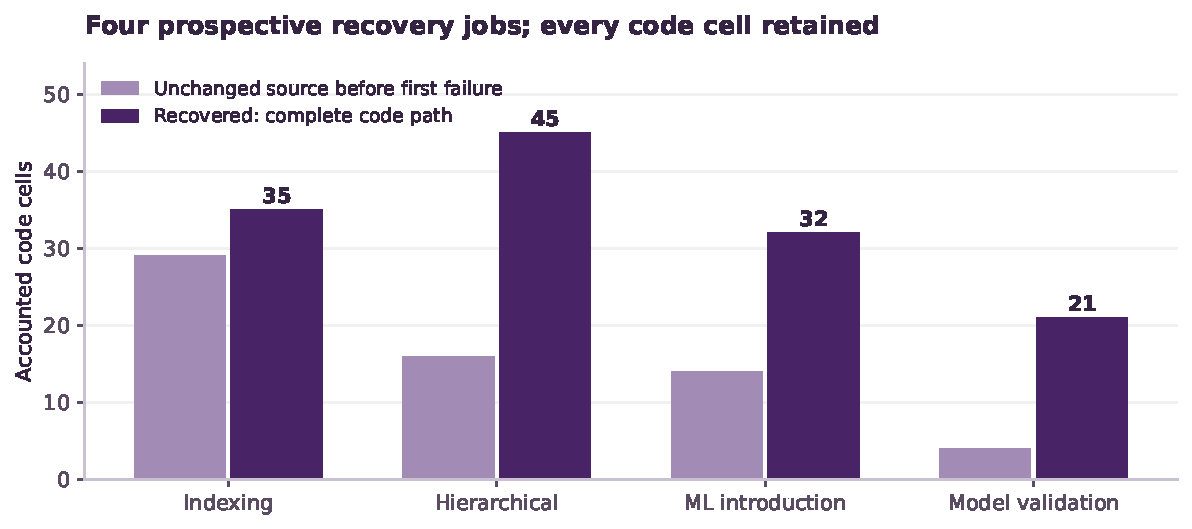
\includegraphics[width=\linewidth]{delivery_completion.pdf}
\caption{Complete recovered code paths. The hierarchical notebook's intentional invalid syntax is represented by an explicit expected-error demonstration, not silently omitted.}
\end{figure}

\subsection{Semantic repair, not execution theater}
Several details matter more than a success flag. The indexing notebook used \texttt{.ix} to mix positional row selection with label-based columns. A blanket substitution would alter behavior. The recovered expression preserves each axis's selection rule, and an explicit sort restores the archived alphabetical table order rather than modern dictionary insertion order.

The hierarchical notebook contains an intentionally invalid slice expression. Recovery retains the original expression as a string, compiles it, catches only the expected \texttt{SyntaxError}, and fails if the expression unexpectedly compiles. Its ordinary grouping calculations are modernized with explicit row and column grouping. Manual independent aggregations verify values, indices and group labels.

The scikit-learn introduction originally downloads Iris from an unpinned endpoint. We freeze an exact current snapshot from the same seaborn-data source and bind its hash. This is not asserted byte-identical to the file downloaded in 2016. The record preserves its relationship to the UCI Iris dataset, whose documentation itself notes historical data differences. The classifier, PCA geometry and digit-classification outputs are checked against the actual supplied inputs \citep{iris,seaborndata}. An initial attempt failed at the read-only default seaborn cache; that environmental failure is retained. The final unchanged-code baseline supplies the same authorized CSV in a writable official cache and then fails at a genuinely removed API.

The hyperparameter notebook requires particular care. Simply deleting the removed \texttt{normalize} option would shrink the specified experiment. Recovery retains all 84 parameter combinations and seven folds. A small estimator adapter implements the documented historical centering and column L2 scaling inside each training fold, ignoring normalization when the intercept is disabled. It uses ordinary current least squares and makes no new numerical-method claim. It is checked against independent polynomial and scale-separated references. Current LAPACK results and seeded illustrative draws are not asserted bitwise identical to old binaries or unseeded historical realizations \citep{legacyregression}.

\subsection{Independent checks, reruns and adverse evidence}
The numerical/semantic checker was authored in a separate agent context from original inputs and mathematical anchors before examining repaired code. This is procedural independence within one team and model family, not an outside audit. It verifies table values and row order; explicit grouped means; PCA geometry using an independent singular-value construction; digit classification through an independent Gaussian calculation; direct nearest-neighbor leave-one-out behavior; the complete parameter grid; and regression behavior under scaling. The check records are identical across the two independent reruns.

Twenty-four source and scope assertions confirm hashes, source-cell mapping, retained order and declared edits. Adverse controls reject wrong critical outputs, altered identities, and errors that occur only while formatting the displayed final value of a cell. Network refusal is also exercised. The initial control harness expected the network attempt to reach its socket hook, but the managed environment denied socket creation earlier. That false control-summary assumption is preserved and corrected to classify the earlier denial; no notebook acceptance changed.

The primary runner explicitly evaluates and represents final expressions. This matters because the development concatenation notebook puts computations inside a display object's representation methods. A bare \texttt{exec} loop that discards the display result could falsely pass it. The independent IPython runner instruments display-time exceptions as failures. Both routes therefore test the actual displayed calculations.

A later visual review found an additional handoff failure: replacing the inline plotting backend with Agg allowed plots from successive cells to accumulate on earlier figures. Numerical acceptance alone had missed the corrupted charts. The initial five introduction figures and two hyperparameter figures are preserved as superseded. Recovery now retains native inline plotting in the notebook, while the CLI captures and closes figures after each cell. Independent figure checks require all nine introduction and seven hyperparameter plotting cells, and the corrected plots are visually inspected. This is a real delivery correction, not an additional successful customer case.

The observed independent execution times were seconds per notebook, excluding process startup and frontier-model work. They are reproducibility measurements, not estimates of all delivery effort or service turnaround. All required plots are generated. The package records exact tested package versions and runnable commands; clean installation in every operating system or a fully archived wheelhouse was not tested.

\section{Frontier execution, configuration and cost boundaries}\label{sec:model}
The actual construction used the available frontier assistant, specialist delegation, read-only repository/web access, local code execution, source inspection, targeted edits, independent checks, recovery and artifact packaging. No new paid API endpoint was invoked. The session identifies the assistant as GPT-6 Astra Pro; an independently exportable inference snapshot, all sampling parameters, reasoning-token totals and a provider invoice are not exposed. That reported interface identity is not treated as proof of a particular billed API configuration.

For deployment costing, we separately verify the public \texttt{gpt-6-astra} documentation and tariff. Standard short-context rates are \$10 per million uncached input tokens and \$50 per million output tokens; the output budget includes reasoning. Inputs above 272,000 tokens in one request trigger higher full-request rates. The documentation lists a 128,000-token output limit. The central initial delivery envelope is eight modeled calls of 250,000 input and 50,000 output tokens each: 2 million aggregate input plus 400,000 output, or \$40 before outcome-specific retry multipliers. All 44 scenario/outcome budget partitions satisfy those per-call caps. These are prospective budgets, not reconstructed usage receipts \citep{astramodel,pricing}.

The primary operating model automates preparation, repair execution, testing and packaging where supported. It does not insert a mandatory manual-review charge. Human time appears only in identified exception resolution, customer support, sales, maintenance and administration. Those quantities are explicit modeled operating requirements, not observed time sheets. A production service would also need approved model access, metering and isolation for customer code; this study does not claim that service is deployed.

No ordinary-versus-expert model trial was conducted with matched prompts, budgets and fresh jobs. Unchanged historical code is an engineering baseline, not an ordinary frontier-model operator. Consequently, the study demonstrates useful delivery but does not establish incremental Operational Alpha. This is an evidence boundary, not a reason to suppress the commercial model.

\section{Human provision, buyer value and price}
\subsection{Equivalent scope, explicit resource estimates}
The human comparison covers the same complete handoff: intake, repair, independent verification, packaging, correction/support and coordination. It is not the price of a broad consulting engagement compared with a tiny automated probe. The central eight-hour estimate allocates one hour to triage, two to repair, two to verification, one to packaging, one to expected support and one to coordination/handoff. Low and high resource totals are four and sixteen hours. These hours are estimates; no timed human control was performed.

Public rates anchor plausible resource pricing. Vanderbilt lists general RSE work starting at \$84/hour, with institutional and complexity qualifications. Notre Dame lists \$149/hour for external engineering services including software/algorithm development. ParaTools lists specialized scientific-computing consulting at \$249/hour unloaded and \$412.97 loaded. Posted rates are not exact quotations for this offer and should not have benefits or overhead added a second time \citep{vanderbilt,nd,paratools}.

\begin{table}[htbp]\centering\small
\begin{tabularx}{\linewidth}{@{}YrrY@{}}\toprule
Reference & Hours & Total & Use and qualification\\\midrule
Low: institutional starting rate, \$84/h & 4 & \$336 & Easy cases / access-dependent alternative\\
Central: external provider, \$149/h & 8 & \$1,192 & Scope-matched estimated engagement\\
High: specialized unloaded, \$249/h & 16 & \$3,984 & Resource reference, not loaded customer outlay\\
High: specialized loaded, \$412.97/h & 16 & \$6,608 & Separate loaded provider reference\\\bottomrule
\end{tabularx}
\caption{Transparent labor-price references. The central \$900 offer is 24.5\% below \$1,192, but substantially above the low reference.}
\end{table}

The model values fractional operating labor at \$95/hour. This is a rounded resource proxy from the BLS developer median and professional compensation ratio: \$135,980/2,080 hours multiplied by \$73.69/\$50.98 gives approximately \$94.50/hour before additional provider overhead or utilization adjustments. It is not an independently contracted wage. The cash model conservatively pays this labor as it occurs \citep{blswage,blsecec}.

\subsection{A participation constraint, not automatic demand}
A low production cost does not determine selling price. A buyer pays for a useful verified result, saved attention, predictable scope and correction responsibility. We test \$500--\$1,500 prices, including a \$600 pressure case and a \$1,200 higher-price sensitivity. The latter is not a validated rush tier or evidence of willingness to pay. No additional demand is silently granted when price falls.

Let $H$ be an adequate human alternative, $P$ the accepted capsule price and $q$ the final acceptance probability. If a rejected capsule is refunded and the buyer then uses the human alternative, expected gross savings are $q(H-P)$, before incremental setup, delay and trust costs. For $H=\$1,192$, $P=\$900$ and $q=0.85$, those costs must fit within \$248.20. For $H=\$336$, the same offer has no price advantage. If a free adequate replacement exists, a labor-cost comparison cannot manufacture a buying reason.

This explains the targeting condition. The offer is plausible for a custom analysis whose output matters and whose cheapest adequate alternative has material engineering cost. It is weak for trivial notebooks, freely maintained examples or tasks a buyer can safely solve with ordinary self-service AI. Competition can reproduce the technical capability and compress price. Differentiation must be earned through responsibility, reliable acceptance, trust and distribution, not asserted exclusivity.

\section{Complete commercial economics}
\subsection{Accounting identities}
Let $N$ be attempted eligible orders over the campaign, $q$ final acceptance after correction/refund, $a$ the initially paid fraction, $P$ the price, $f$ the proportional payment fee, $b$ its fixed part, $c(q)$ expected direct delivery cost per attempt including failed work, $k$ acquisition cost per attempt, $F$ attributable fixed operating cost and $D$ additional development. Then
\begin{align}
R &= NqP,\\
\Pi_{\mathrm{direct}} &= NqP-Nc(q)-Na(fP+b),\\
\Pi_{\mathrm{operating}} &= \Pi_{\mathrm{direct}}-Nk-F,\\
\Pi_{\mathrm{project}} &= \Pi_{\mathrm{operating}}-D.
\end{align}
The paid fraction can exceed final acceptance because the original processing charge is retained on later-refunded payments. No customer cash is called accepted revenue before the modeled acceptance outcome. The full-project break-even price at positive volume is
\begin{equation}
P^* = \frac{c(q)+k+(F+D)/N+ab}{q-af}.
\end{equation}
The implementation recomputes the outcome mix, correction expense and payment exposure when acceptance changes. It does not lower quality while holding every associated cost fixed. For a fixed purchased inquiry campaign, acquisition is charged even if no inquiries convert, rather than dividing by nonexistent orders.

\subsection{Joint delivery outcomes and cost coverage}
The central outcome mix is 60\% clean acceptance, 25\% corrected acceptance, 12\% rejection before payment and 3\% later full refund. Thus $q=0.85$ and $a=0.88$. Each outcome carries different model/retry, tool, support and exception costs. The probabilities are transparent commercial assumptions, not frequencies estimated from the four selected cases. The expected model charge is \$53.80 per attempted job after retry multipliers, with tools, retention and genuine human intervention bringing direct expense to \$84.3825 per attempt.

Acquisition assumes 40 qualified inquiries monthly at \$25 each, including 0.1 hour of sales attention valued at \$95 and \$15.50 channel expense. A 20\% purchase conversion gives eight attempts, \$125 acquisition per attempt and \$147.06 per finally accepted outcome. These are unmeasured channel assumptions. Monthly fixed expense is \$900: four maintenance hours, four administration hours, \$60 hosting/software and \$80 business services. Additional development is forty hours plus \$200 tooling, totaling \$4,000. Delivery work is charged once; knowledge acquired while doing it does not incur a duplicate research bill.

The model includes rejected jobs, retries, checking, correction, packaging, support, acquisition, payment charges, maintenance and infrastructure. The payment benchmark is the U.S. domestic-card 2.9\% plus \$0.30, varied in sensitivity; it is not asserted to be the tariff of a Canadian account \citep{stripe}. The baseline assumes complete collection of earned invoices, zero bad debt and equity financing. Credit-loss/dispute sensitivities and delayed collection are reported separately. No debt interest, realized taxes, market-size forecast or corporate valuation is silently inferred.

\subsection{The central result}
\begin{table}[htbp]\centering\small
\begin{tabularx}{\linewidth}{@{}Yr@{}}\toprule
Twelve-month central campaign & USD\\\midrule
Accepted revenue: 81.6 expected final outcomes at \$900 & 73,440.00\\
Direct delivery, including unsuccessful attempts & (8,100.72)\\
Payment fees, including initial payments later refunded & (2,230.27)\\\midrule
Direct delivery contribution & 63,109.01\\
Acquisition & (12,000.00)\\
Attributable fixed operations & (10,800.00)\\\midrule
Operating profit & 40,309.01\\
Additional commercial development & (4,000.00)\\\midrule
\textbf{Full modeled project return} & \textbf{36,309.01}\\\bottomrule
\end{tabularx}
\caption{Complete central accounting. Fractional accepted counts are expectations, not fictitious partial customers. All revenue and profit in this table are modeled.}
\end{table}

\begin{figure}[htbp]\centering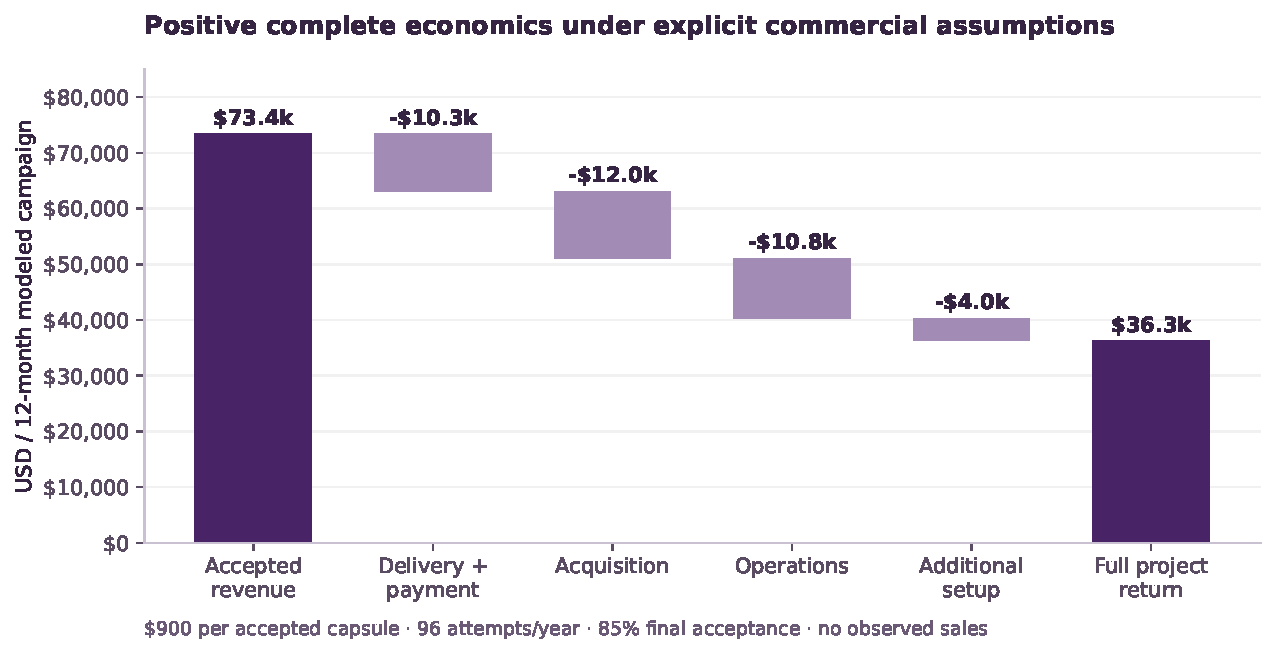
\includegraphics[width=\linewidth]{commercial_waterfall.pdf}
\caption{The positive result survives direct delivery, failed work, acquisition, operations and additional setup. It depends on the stated order, acceptance and cost assumptions.}
\end{figure}

The operating break-even price is \$390.73; the full-project price is \$441.26 at central volume and quality. Current complete project cost is \$455.04 per accepted outcome at the \$900 price. These are different quantities because payment expense itself falls at a lower selling price. With acquisition proportional to orders, the central \$900 offer requires 1.69 attempted orders monthly to cover operations and 2.32 to repay setup over the twelve-month model. Those rates correspond to 1.44 and 1.97 expected final accepted outcomes per month.

If instead 40 inquiries are purchased regardless of conversion, break-even conversion is 7.23\% for operations and 8.49\% for the full project, compared with the central 20\% assumption. The model's maximum operating break-even acquisition cost is \$544.89 per attempt, versus the assumed \$125. This is available economic room, not evidence that customers can actually be acquired at any stated cost.

\section{Sensitivity, capacity and the cash needed to deliver}
\subsection{Joint downside and competitive pressure}
\begin{table}[htbp]\centering\small
\begin{tabularx}{\linewidth}{@{}Yrrrr@{}}\toprule
Scenario & Price & Attempts/mo & Final accept. & Project return\\\midrule
Joint downside & \$600 & 3 & 50\% & $-\$28,943$\\
Central conditional & \$900 & 8 & 85\% & $+\$36,309$\\
Favorable conditional & \$900 & 15 & 95\% & $+\$116,444$\\
Price pressure, other central inputs & \$600 & 8 & 85\% & $+\$12,564$\\
Low uptake & \$900 & 0.5 & 85\% & $-\$13,856$\\
Funded campaign, no sales & \$900 & 0 & --- & $-\$26,800$\\\bottomrule
\end{tabularx}
\caption{A model can support a commercial opportunity without supporting a sales forecast. The downside increases delivery effort and acquisition burden while reducing price, quality and volume.}
\end{table}

The downside is not a single parameter perturbation: higher frontier consumption and retries combine with lower acceptance, demand and price, and \$8,200 setup. Direct contribution is already negative; volume cannot repair an unprofitable attempted-job margin in that configuration. At the other extreme, the favorable case assumes supported tasks and repeat/channel efficiencies; these are not measured learning gains. The \$600 scenario holds volume and quality constant, making it a clear price-pressure test rather than a demand curve invented to preserve profit.

\begin{figure}[htbp]\centering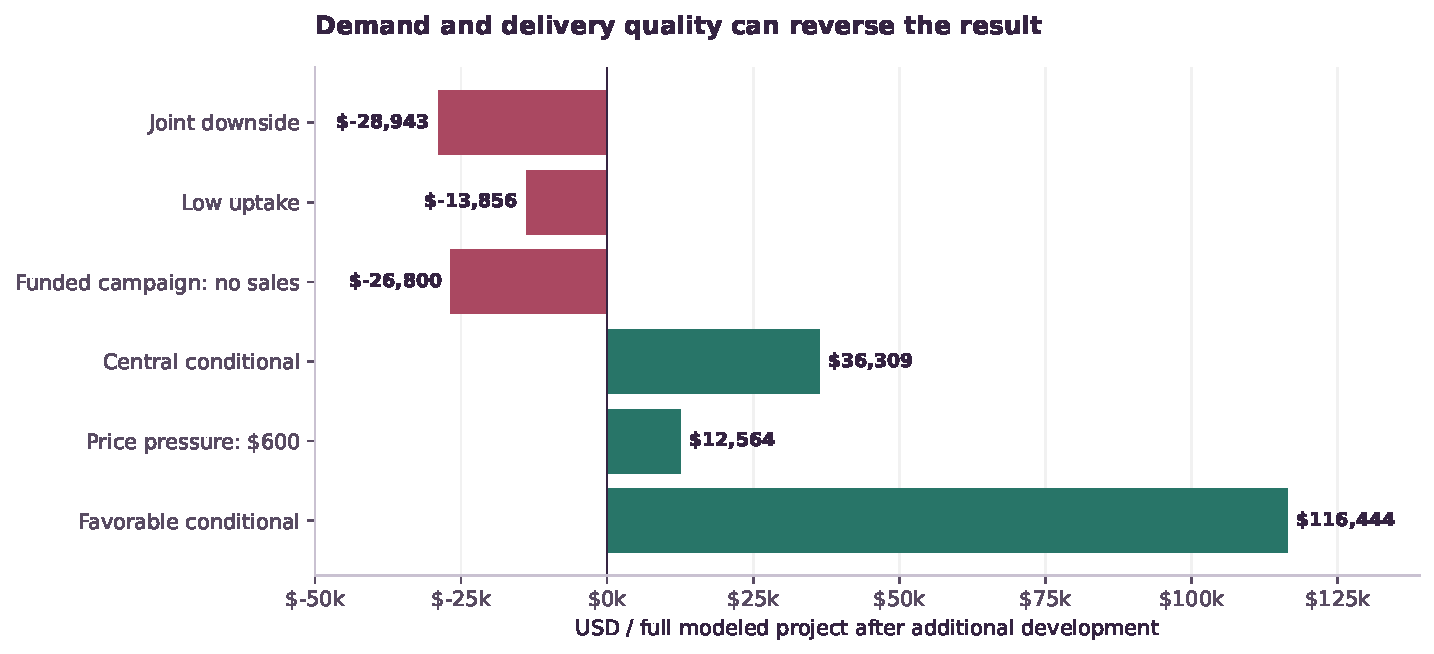
\includegraphics[width=\linewidth]{scenario_results.pdf}
\caption{Full-project outcomes under alternative commercial arrangements. A campaign with no sales still pays for acquisition and operating availability.}
\end{figure}

The central mix-adjusted acceptance threshold is 40.58\% for operating profit and 44.99\% for full-project recovery. At 40.1\%, the full result is $-\$4,434.29$; at 44.9\%, $-\$78.66$; at 45.0\%, $+\$12.09$. The first two stress levels are informed by the revised broad-corpus MLEModernizer results, but are not matched population estimates. Their proximity to the break-even threshold is material: the central 85\% assumption must be validated on real screened customer jobs before relying on the forecast.

\begin{figure}[htbp]\centering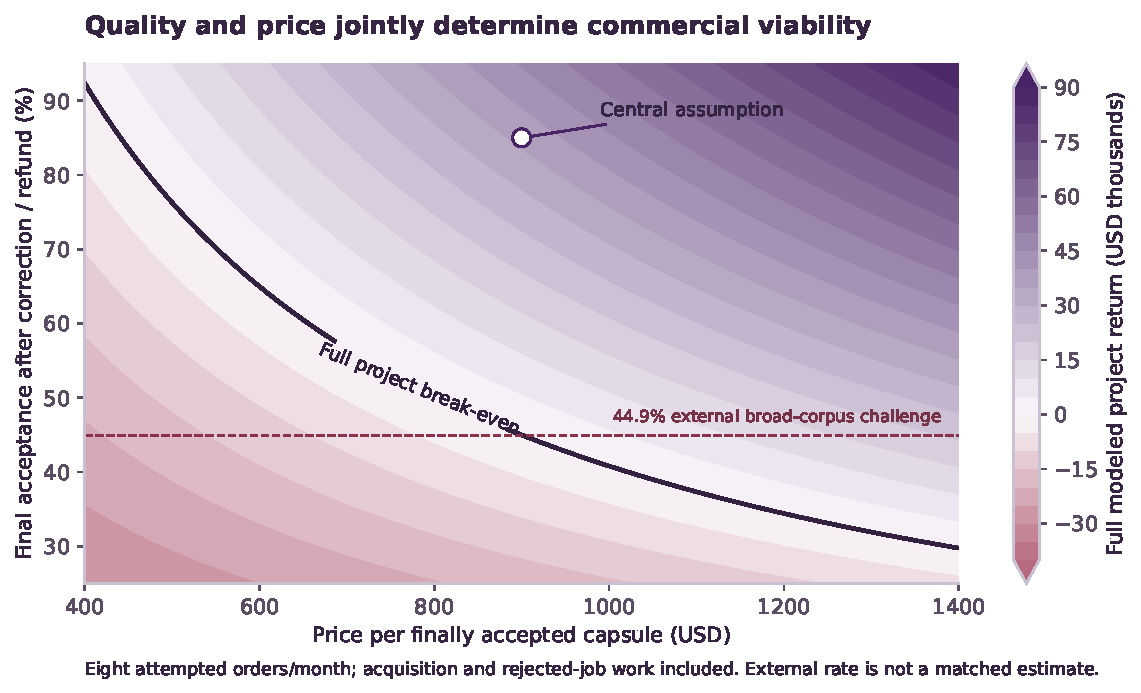
\includegraphics[width=\linewidth]{commercial_frontier.pdf}
\caption{A conditional viability frontier at eight attempted orders monthly. Final acceptance changes rejection, correction and payment cost jointly. A point above the frontier is not evidence that buyers exist.}
\end{figure}

The package includes a 1,001-cell deterministic parameter grid and 1,000 seeded histories with an explicitly assumed 10\% monthly common-incident rate. An incident reduces volume and quality while increasing model expense. The reported distributions are conditional simulation outputs; neither their positive fraction nor their quantiles are real-world profitability probabilities or statistical confidence intervals. Price, paid demand, acceptance, acquisition and additional development are the dominant unresolved commercial variables.

\subsection{Capacity without an invented full-time team}
The central model uses 14.42 human hours monthly: eight for maintenance/administration, four for acquisition and 2.42 for support and exception work. It assumes a fractional shared operation rather than hiding a full dedicated salary. Under the stated 40 available human hours and 160 available agent hours, the nominal capacity envelope is 39.88 attempted jobs per month. The tested 3--15 order scenarios fit that envelope. API rate limits, actual duration tails, sales-response queues and the proposed two-business-day service level were not operationally measured. Capacity is therefore an explicit planning constraint, not a throughput claim.

\subsection{Profit and financeability are separate}
The default payment arrangement collects on initial acceptance and reserves every receipt still exposed to the 14-day warranty. Refund reserves are restricted cash, not a duplicate expense. Expected-case opening equity of \$6,760.92 covers setup, operations, acquisition, delivery and timing before unrestricted receipts accumulate. The cash model uses a conservative five-calendar-day delivery buffer; that is a liquidity assumption and does not replace the proposed two-business-day offer.

If all eight jobs in the first cohort are initially paid and then fully refunded after failed correction, opening cash rises to \$10,298.12, assuming later cohorts recover to central conditions. A 35-day collection delay requires \$9,003.82. These are conditional equity requirements, not financing commitments or tail-risk solvency guarantees. A fully restricted 50\% deposit does not fund production; delayed collection until the warranty closes changes fees and timing without weakening the customer's promised outcome. Sixteen event ledgers reconcile cash, refunds and reserves through modeled runoff.

\begin{figure}[htbp]\centering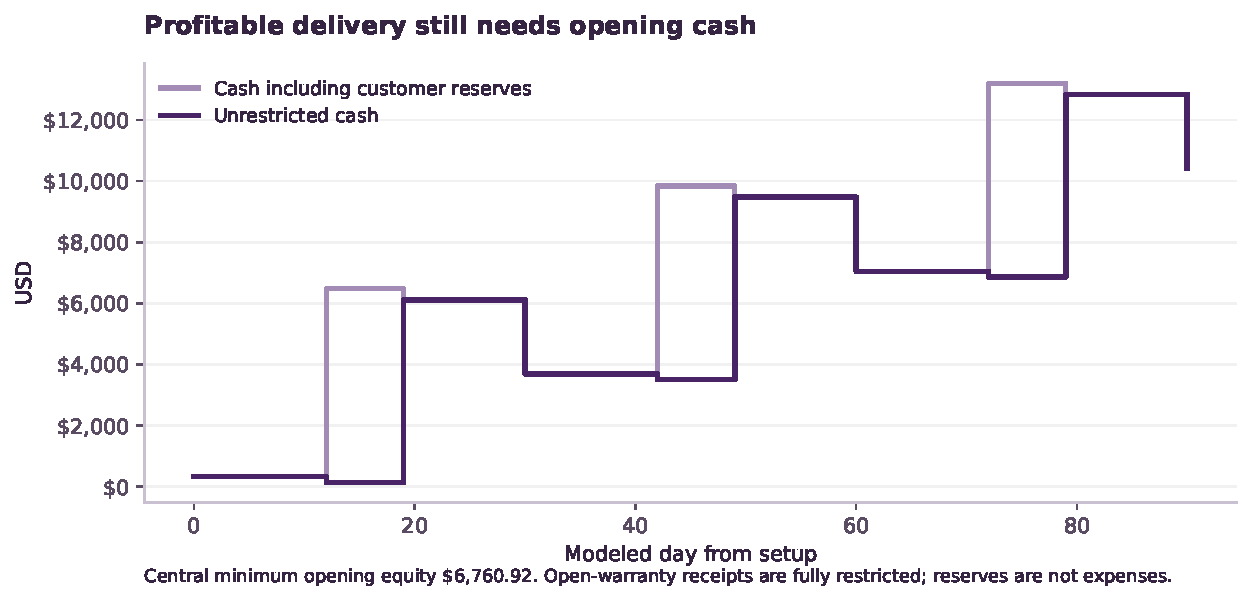
\includegraphics[width=\linewidth]{cash_reserves.pdf}
\caption{The cash account is not the spending account. Central first-quarter flows show the gap between total cash and funds available after customer reserves.}
\end{figure}

\section{Complementarity, optional Alpha and ecosystem execution}
\subsection{Sharing is tested as an additional choice}
The primary offer does not need a retained skill or shared arrangement to be worthwhile in the central model. An auxiliary factorial comparison considers human provision and frontier-assisted provision, each with and without ordinary shared work. Cohorts of four, eight and sixteen jobs receive the same assumptions: 15\% reusable-work benefit, \$380 setup, half an hour plus \$20 coordination per cohort, allocated across its jobs, and 5\% common rework exposure. Reuse requires participant permission and compatible rights.

At four jobs, coordination worsens both arrangements. At sixteen jobs, the competent human shared arrangement saves resources, while the assumed AI reuse benefit still fails to repay coordination. This is an illustrative commercial complementarity test, not observed retained Alpha. An early auxiliary table incorrectly used a provider selling-price anchor as in-house production cost. It is preserved and superseded by a table using eight hours at the same \$95 resource proxy as other labor. The main commercial results were unaffected.

No Gym development, weight update or extra extraction investment was admitted. The notebook adapter and checks are ordinary reproducible software assets. Without a matched fresh-recipient trial against both a competent baseline and an ordinary library containing the same asset, there is no supported retained-Alpha claim. Retaining useful source files for reproducibility is not itself evidence of a self-accelerating network.

\subsection{Existing components were reused, with their boundaries intact}
Twenty-six unchanged repository files, including licenses, are copied and verified against their Git blob and SHA-256 identities before use. The study executes the native Nova-Seed sealing/opening path and rejects a ciphertext modification. FusionPlan compiles and verifies six job specifications and rejects a modified success specification. Insight validates the discovery packet and returns an evidence-needed state. These executions connect the job, source, deliverable and evidence identities without inventing a parallel runtime.

The native cost schema validates 54 records whose accrued actual costs remain unknown, and rejects an attempted unknown-to-zero conversion. The study does not initialize signed CostLedger admission or assert a complete actual-profit seal. MARK is \texttt{NOT\_EXECUTED}; live ENS authentication and settlement are \texttt{NOT\_EXECUTED}. A local test passphrase is a public fixture, not a live identity credential. Nominal AGIALPHA job fields demonstrate the existing schema and are neither USDC receipts nor commercial revenue. Cryptographic integrity does not establish scientific correctness, customer utility or demand.

\begin{table}[htbp]\centering\small
\begin{tabularx}{\linewidth}{@{}p{.25\linewidth}Yp{.23\linewidth}@{}}\toprule
Question & Supported result & Current status\\\midrule
Commercial foundation & Verified useful sample; positive complete economics under stated price, demand and acceptance & Conditional positive\\
Operational Alpha & No matched ordinary/expert frontier trial & Unestablished\\
Retained Alpha & Ordinary assets retained; auxiliary sharing does not justify extra investment & Not admitted\\
Transformational discovery & Customer-specific recovery arrangement investigated; modernization prior art and free substitutes recognized & Bounded opportunity, no exclusive technical novelty\\\bottomrule
\end{tabularx}
\caption{The four conclusions remain separate. Failure to establish optional Alpha does not negate a conditional profitable service.}
\end{table}

\section{Expansion through earned productive capacity}
The immediate result is six delivered engineering packages and a priced, bounded offer that can be assessed without buying a speculative physical product. Its next commercial stage would require authorized access to real customer-specific notebooks, a concrete purchase decision, metered delivery and acceptance records. The first measurements should target the model's weakest links: conversion, complete job cost, final acceptance, support burden and cash collection. The thresholds above make those observations decision-relevant.

If those measurements support the service, recurring work could consist of a maintained notebook portfolio with scheduled compatibility checks and explicitly priced recovery events. Additional offerings could package validated data transformations or analytical methods for repeated internal use, provided the original rights allow it. A customer remains free to take the delivered code elsewhere; portability can reduce switching anxiety, but does not create a moat. Distribution and reliable responsibility would have to earn repeat purchase.

Shared capabilities should follow actual reuse demand. A maintained adapter or test library deserves incremental investment only when fresh-job benefits exceed extraction, validation, support and coordination costs. The present auxiliary result warns against assuming that every capability should be shared. A conventional library with the same content is an essential comparator. Larger capacity would require measured queue performance, more working capital, support coverage, stronger production isolation and model-access continuity; the current fractional-operation economics cannot be extrapolated to an unlimited service.

The long-term ambition is an enterprise that converts useful intelligence into durable productive capacity, then uses that capacity to pursue additional consequential work. Restoring a neglected analysis is a small, testable instance of that direction. A path to broader infrastructure must be built from accepted useful outcomes, reproducible capabilities and responsible capital deployment. One conditional service margin provides neither a valuation formula nor evidence of economy-wide transformation.

\section{Limitations that govern the conclusion}
The commercial answer is conditional because the paying population is unobserved. The purposive same-author teaching sample is easier and more available than many abandoned research projects. Its four successes cannot support a population confidence interval or the assumed 85\% final customer acceptance. A free updated edition substantially weakens willingness to pay for these exact examples. The study therefore supports construction feasibility and a conditional unit of sale, not a demonstrated underserved market at measured scale.

Independent checking reduces specific semantic risks, but the checker and repairer belong to the same team and model family. Shared blind spots remain possible. Current source fixtures and seeded randomness are explicit; bitwise recreation of every historical output is not promised. Neither scientific correctness of the underlying analysis nor the proposed service-level agreement follows from the runtime checks.

Actual model charges and complete actual study cost are unknown. Documented API prices and explicit budgets make the deployment model auditable, but they are not a measured cost advantage over human providers or ordinary AI. Human hours, support, acquisition and volume are estimated. The primary model pays fractional labor, assumes equity funding and includes modeled obligations, but actual legal/tax/accounting arrangements and customer contracts do not exist in this study.

The package is a pinned research review edition. Full code/data/HTML qualification and canonical publication remain with the existing repository route and owner. A downloadable HTML file is not a deployed customer service. The source-only scope avoids changes to existing runtimes, catalog, homepage, workflows, versions or production permissions \citep{publication}.

\section{Conclusion}
AGI ALPHA has produced a concrete useful digital outcome and a positive, fully costed conditional commercial result for a bounded recovery offer. Four prospective notebooks pass complete execution and separately authored checks; the central \$900 arrangement produces \$36,309 after additional development over twelve modeled selling months. The result survives inclusion of failed attempts, correction, acquisition, support, operations and cash reserves.

The evidence also gives clear failure conditions. Low uptake, heavy correction, an adequate free substitute or acceptance near the adverse broad-corpus reference can eliminate surplus. Those conditions are preserved rather than repaired by changing the headline requirements. The next claim to earn is paid repeatability on the actual target population. Operational Alpha, retained skills and wider transformation remain optional additional achievements, each requiring its own evidence.

\clearpage
\appendix
\section{The recorded opportunity shortlist}\label{app:shortlist}
The search log is retained in \texttt{evidence/selection\_review.json}. The following summarizes the three candidates without treating hypothetical price ranges as observed market prices.

\subsection{Selected: customer-specific analytical recovery}
\textbf{Beneficiary and need:} a small research or R\&D team whose inherited analysis cannot be rerun or safely extended. \textbf{Outcome:} a complete rerunnable notebook/CLI, provenance, semantic checks and correction responsibility. \textbf{Existing limitation:} bespoke repair can require specialist interpretation and coordination; tooling assumes varying degrees of preparation and does not universally establish scientific correspondence. \textbf{Why agent execution may help:} source reasoning, execution feedback and verification can be combined repeatedly within one bounded job. \textbf{First artifact:} the six delivered code-only capsules. \textbf{Human reference:} explicit four/eight/sixteen-hour resource cases and documented provider-rate anchors. \textbf{Buying reason and price:} access to useful custom analysis and less uncertain engineering effort; \$500--\$1,500 modeled range, conditional on adequate alternatives. \textbf{Cheapest falsifier:} one admitted task whose required outputs cannot be preserved, or a prospect with a cheaper adequate substitute. The engineering falsifier was tested; purchase preference was not.

\subsection{Deferred: accessible STEM-diagram bundles}
\textbf{Beneficiary and need:} blind or low-vision learners and specialist educators facing unavailable accessible technical diagrams. \textbf{Outcome:} structured descriptions, editable tactile vectors, labels and a semantic map whose content a reader can use. \textbf{Existing limitation:} generic image conversion does not assure correct topology, scale, terminology or comprehension; established specialist standards and libraries already exist. \textbf{Why agent execution may help:} domain interpretation can be combined with exact vector construction and consistency checking. \textbf{First artifact:} one licensed diagram in multiple access formats. \textbf{Human reference:} a transparent but unvalidated 10--24 hours at \$50--\$100/hour for a ten-figure bundle. \textbf{Buying reason and price:} timely access to otherwise missing material; \$500--\$1,200 hypothetical range. \textbf{Cheapest falsifier:} a qualified touch-reader comprehension test. No such user was available, so the consequential acceptance criterion could not be established here.

\subsection{Deferred: legacy instrument-data reuse}
\textbf{Beneficiary and need:} a small laboratory with raw exports that cannot be used across available analysis tools. \textbf{Outcome:} a validated conversion with units, sample identity, metadata and reconstruction evidence. \textbf{Existing limitation:} file parsers and standards exist, but missing local calibration and semantics can defeat correct interpretation. \textbf{Why agent execution may help:} heterogeneous documentation, existing parsers and independently checked adapters can be assembled into a handoff. \textbf{First artifact:} a licensed spectral fixture converted with round-trip checks. \textbf{Human reference:} unvalidated eight--24 hours at \$80--\$150/hour. \textbf{Buying reason and price:} reuse without a specialist migration engagement; \$700--\$2,000 hypothetical range. \textbf{Cheapest falsifier:} missing units or calibration essential to the promised decision. Representative customer files were unavailable; conversion alone could not establish this value.

\section{Preserved failures and corrections}
\begin{longtable}{@{}p{.23\linewidth}p{.36\linewidth}p{.34\linewidth}@{}}
\toprule
Record & What failed or was limited & Resolution and impact\\\midrule
\endhead
Original notebook executions & Removed APIs prevent full completion in each of six cases & Original inputs and first-failure logs retained; no injected bugs\\
Development checker hook & Local import shadowing prevented checks despite full execution & Acceptance withheld; code fixed; failed records and successful reruns retained\\
Initial seaborn baseline & Read-only default cache failed before relevant API drift & Same-source fixture supplied in writable official cache; original code then fails at removed split API\\
Plot lifecycle & Headless backend merged independent cell plots despite numeric passes & Preserve bad figures; restore inline lifecycle; verify nine/seven expected plot cells and rerun numeric checks\\
Historical Iris identity & Original notebook used an unpinned URL & Bind current same-source snapshot; do not claim 2016 byte identity\\
Intentional invalid syntax & Source includes a pedagogic SyntaxError & Exact invalid expression retained in an expected-error test; not silently omitted\\
Hyperparameter modernization & Deleting normalize would remove half the experiment & Preserve all 84 settings and training-fold normalization semantics\\
Network control expectation & Environment blocks socket creation before hook records a connect & Preserve false harness summary; classify earlier refusal correctly\\
Auxiliary coordination price & Provider selling price used as internal resource cost & Superseded table preserved; corrected \$95/hour proxy; main result unchanged\\
Unsuccessful sales campaign & No-inquiry scenario did not cover funded acquisition with no conversion & Added full \$26,800 loss case\\
API aggregate budget & Aggregate tokens alone did not prove per-request pricing eligibility & Added 44 explicit bounded request partitions\\
Current prior art & Older favorable recovery headline superseded by revised result & Use 40.1\%/44.9\% reference challenges; no unsupported superiority claim\\
Independent model Alpha & No matched ordinary/expert deployment trial or metered billing & Keep unestablished; do not turn missing Alpha into a commercial veto\\\bottomrule
\end{longtable}

\clearpage
\section{Full assumption map and reproducibility}
\subsection{Evidence levels of the economic inputs}
\begin{longtable}{@{}p{.27\linewidth}p{.29\linewidth}p{.37\linewidth}@{}}
\toprule
Input & Central value & Evidence level / source\\\midrule
\endhead
Supported artifact & One notebook, at most 100 code cells and 5 MB input & Frozen offer; four confirmation cases execute\\
Selling price & \$900 per final accepted outcome & Proposed price, not an observed purchase\\
Qualified inquiries & 40/month & Unmeasured demand assumption\\
Purchase conversion & 20\% & Unmeasured; funded-campaign threshold reported\\
Final acceptance & 85\% & Unmeasured customer outcome mix; not inferred from 4/4\\
Initial payment & 88\% & Includes 3\% later full refunds\\
Baseline API & 2M input + 0.4M output; \$40 & Documented rates, modeled usage; eight bounded calls\\
Model cost after retries & \$53.80 per attempt & Joint outcome multipliers, not a bill\\
Direct expense & \$84.3825 per attempt & Includes tools, retention, support, exceptions and failure\\
Human resource proxy & \$95/hour & Rounded wage/compensation estimate; cash-paid model\\
Acquisition & \$25 per inquiry / \$125 per attempt & Includes sales labor once plus modeled channel expense\\
Fixed operation & \$900/month & Maintenance/admin eight hours plus services/hosting\\
Additional setup & \$4,000 & Forty additional hours plus \$200 tooling\\
Payment fees & 2.9\% + \$0.30 & U.S. reference; other fee cases included\\
Collection / warranty & Initial acceptance / 14 days & Modeled terms; reserves fully restricted\\
Income tax / debt & Not modeled / equity financed & Profit is before income tax; no debt commitment\\
Actual collections & \$0 & No customers or external payments\\
Actual complete cost & Unknown & Session has no complete usage/invoice record\\\bottomrule
\end{longtable}

\subsection{Reproduction contract}
The top-level \texttt{README.md} describes the exact commands. From the study root, \texttt{python} \path{scripts/reproduce.py} verifies source identities, runs delivered notebooks and independent checks in fresh processes, regenerates economic outputs and produces a reconciliation report. It does not require model calls, customer accounts, credentials or network access for the computation. The documented package environment must already be installed; automatic clean installation and universal platform compatibility are not claimed.

\texttt{python economics/run\_economics.py} reruns the standard-library economic study. Inputs, scenario grids, sensitivities, daily cash ledgers, simulation seeds and independently checked arithmetic are included. A prior complete economics edition is preserved under \texttt{economics/prior/}; amendments carry their reason and new input hash. \texttt{python scripts/native\_evidence\_demo.py} reexecutes the exact-source native integrations. Randomized encryption changes ciphertext across runs while preserving the checked plaintext binding.

The LaTeX publication compiles with \texttt{pdflatex}, \texttt{bibtex}, and two further \texttt{pdflatex} passes in the publication directory. A complete offline browser edition is generated from the same manuscript body with embedded figures and native MathML. Source, bibliography, figures, executive brief, LinkedIn approval draft, run instructions and the complete package are supplied. Each released file is recorded in a SHA-256 manifest. Every final PDF page is rendered and visually inspected.

\section{Claim-to-evidence register}
\begin{longtable}{@{}p{.25\linewidth}p{.39\linewidth}p{.29\linewidth}@{}}
\toprule
Claim & Evidence location & Boundary\\\midrule
\endhead
Useful complete recovery & \texttt{deliveries/}; independent first/second case logs & Four prospective engineering analogues, not paying customers\\
133 cells / 38 checks & \path{evidence/independent_review.txt}; checker and expectations & Repeated runs are not new jobs\\
Source and scope preserved & Source manifests; identity audit; per-case diffs & MIT code only; original prose excluded\\
Adverse failures rejected & Independent controls and preserved first control summary & Bounded controls, not universal robustness\\
\$36,309 full project & \path{economics/results/summary.json}; verification & Conditional price/demand/quality/cost assumptions\\
\$441.26 break-even & Economic model and threshold outputs & Central volume/cost mix; fees depend on price\\
Human \$1,192 reference & Eight-hour breakdown; provider-rate sources & Estimated hours, not a human experiment or quote\\
Liquidity and refunds & Sixteen daily ledgers and reserve checks & Expected cash cases; tail risk not calibrated\\
Frontier configuration & Model record and official model/pricing sources & Actual session billing/snapshot incomplete\\
Native integration & \path{evidence/native_execution.json}; upstream manifest & Local provenance/plan validation; no authority or truth proof\\
Operational / retained Alpha & Explicit absence of matched uplift/transfer test & Not established or necessary for central economics\\
Published status & \texttt{PUBLICATION\_STATUS.json} and immutable review PR & Review source edition; canonical release remains qualification-gated\\\bottomrule
\end{longtable}

\subsection{Publication and responsibility}
This edition follows the existing source/evidence review route, not the passive-paper-only overlay. Code and HTML require normal source qualification before canonical catalog or deployed-experience admission. The branch is additive; original papers and other owners' work remain intact. Public source and attachment links are verified before being described as available. A pinned review edition is explicitly distinguished from a merged canonical release \citep{publication,coordination}.

The study's first obligation is to answer whether the offering delivers a useful result and can cover complete costs at a credible price. The executed handoffs and conditional economics answer that question constructively. They also specify exactly which additional observations would change the decision. That is the basis on which further productive capacity can be earned.
